\documentclass[12pt]{article}
\usepackage{fullpage}
\usepackage{amsmath}
\usepackage{graphicx}
\usepackage{enumerate}
\usepackage{float}
\usepackage{listings}
\usepackage{longtable}
\usepackage[table]{xcolor}
\usepackage{tabularx}
\usepackage[round]{natbib}
\restylefloat{figure}
\title{Project Proposal: Gamifying the transcriptome}
\author{Chidube Ezeozue and Joel Brooks}

\begin{document}
\bibliographystyle{apalike}
\renewcommand\refname{Bibliography}
\maketitle

\section*{Introduction}
The reviewers of our first proposal primarily concerned with the specifics with our game implementation. In this revised proposal, we added more detail about specific elements of the game in order to address these concerns.
Furthermore, we clarified the main use case of our game in the \emph{Innovation} section of this proposal, as it seemed we weren't clear in our first proposal about how the game could be best utilized for contributing to the field.

\section*{Specific Aims}
Our primary goal for this project is to create a game that can potentially utilize human powered computation to reconstruct transcripts and their relative abundance from short RNA sequence reads. We hope to accomplish this by creating a puzzle game that allows users to try and create transcripts and assign abundances to them to explain levels of exon abundance found by RNA-seq technology. In this game, the underlying biology would be abstracted away by representing relative levels of exon abundance within a gene as colored blocks, and thus the game would be designed to be appealing to those with no knowledge of the underlying biological problem they are solving. This game would not be a complete replacement for existing computational methods for transcript assembly as these algorithms have been shown to work well in many cases, but instead utilizing human powered computation to explore the solution space of transcript isoforms in cases where existing algorithmic techniques may be lacking in accuracy.

\section*{Research Strategy}

\subsection*{Significance}
Alternative splicing is an important functional element in eukaryotes \citep{pan2008deep}. These splicing events allow a single gene to produce multiple mRNA transcripts and thus increased biological complexity, as different isoforms may lead to different proteins or different regulation of the same protein \citep{trapnell2010transcript}. These events are quite common, and evidence suggests they occur in roughly 95\% of multiexonic human genes.

The development of RNA-seq technology has greatly advanced the potential effectiveness of mRNA transcript assembly, but detecting isoforms from the millions of short reads generated by RNA-seq is a computationally daunting problem. Currently existing methods are able to asses relative exon abundance for a gene from RNA-seq data with relatively high accuracy \citep{trapnell2009tophat}, however reconstructing the set of mRNA isoforms that produced those exon abundances is a computationally complex problem. Cufflinks uses weighted bipartite graphs in order to find the minimum set of transcripts that explain the set of reads, however, we would like to explore the possibility of humans finding alternative sets of transcripts through a game like interface. The human solutions could then be scored against existing databases of transcripts for genes.

\subsection*{Innovation}
Human powered computation has been shown to be of use in biologically related problems \citep{kawrykow2012phylo, cooper2010predicting}. For example, Phylo allowed humans with no understanding of biology to perform multiple sequence alignment (MSA). Phylo was designed to abstract the underlying biology away by representing nucleotide bases as colored blocks.  The intuition behind such an abstraction is humans are quite good at visual pattern recognition problems. Using Phylo, humans were indeed able to outperform state of the art MSA algorithms for certain sequences. We'd like to use similar motivation for exploring the idea of humans reconstructing transcript isoforms from relative abundances  of exons. We believe that this problem can effectively be conveyed in a simple block-based puzzle, and therefore a person with no understanding of computation or biology can play but still potentially find useful solutions. Thus, by abstracting the problem of transcript assembly into a simple puzzle form, we can hopefully use human powered computation to help parse RNA-seq data. Due to the overhead of human powered computation, utilizing our game for complete transcriptome assembly would be difficult. However, we envision
this project being utilized in a similar manner to Phylo, where solutions to complex regions can be explored by humans and compared to those found by the current gold standards.

\subsection*{Approach}
\subsubsection*{Data preprocessing}
For our game we intend to use genomic data from the mouse to ease comparison with related work given that most other authors in this area worked with the mouse genome \citep{trapnell2010transcript,guttman2010ab,feng2010inference,li2011isolasso}. Since read alignment and exon detection is outside the scope of this project, we would use the tool TopHat \citep{trapnell2009tophat} to perform these tasks. The input to the game would therefore be expression levels for the different exons and junctions in the mouse genes. \\
However, to be able to stratify the game into difficulty levels we would organize the genes by number of exons and amount of disagreement on genes' isoforms using other tools. \\
After pre-processing the reads with TopHat, we would push exon and junction expression level data to a database for easy retrieval. We chose to use a database since the voluminous read data is not relevant to our problem and therefore not useful to store.
\subsubsection*{Game Development}
Our game would have 2 major components:
\begin{enumerate}
\item A backend for supplying challenges to players and aggregating their solutions. We would build this backend using a Python/Django webserver and a MySQL database or Google App Engine datastore.
\item The actual game would be built as either a Java desktop application or browser-based game. In either case, our proposed user interface is demonstrated in Figure \ref{fig:proposedui}
\begin{figure}[H]
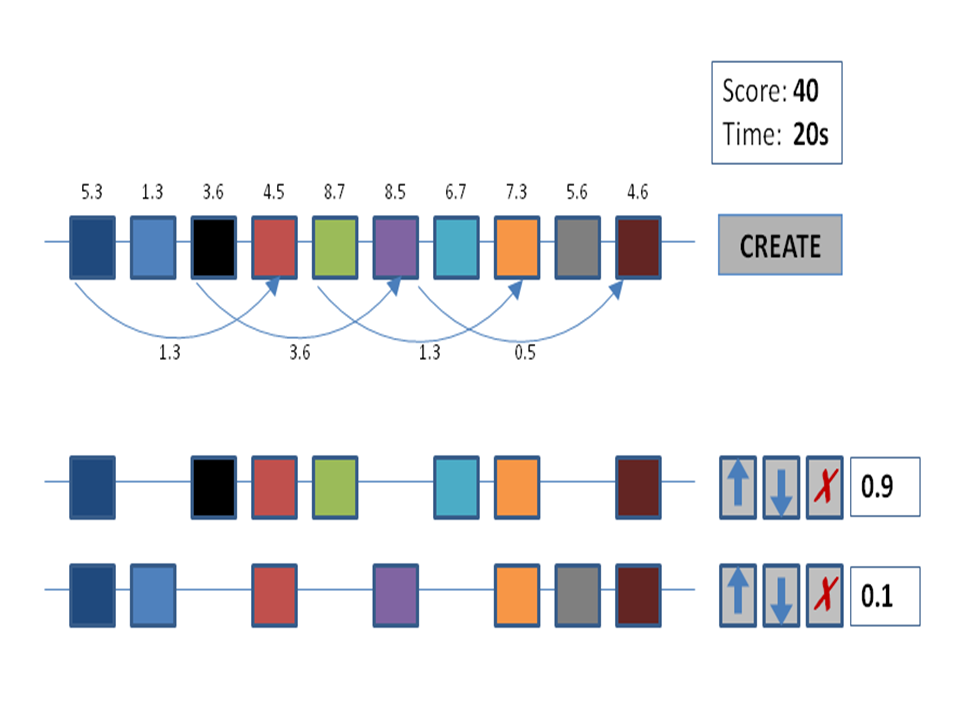
\includegraphics[scale=0.5]{ProposedUI.png}
\caption{Proposed user interface of transcriptome assembly game}
\centering
\label{fig:proposedui}
\end{figure}
When the game starts, players will be presented with a gene where each column of blocks represent exons discovered by TopHat, and column heights represent their relative abundances. Furthermore, columns will contain ``linked" boxes that contain a unique identifier shared with a box in another column.
These represent reads that mapped to more than one exon and spanned a splice junction. Players will then be able to copy this entire gene into a transcript, delete exons and vary the relative expression levels of their transcripts in order to remove boxes from the puzzle. ``Linked" boxes can only be removed by
transcripts that contain both exons corresponding to the ``linked" boxes without the exons in between them. Players will be scored using the following criteria:
\begin{itemize}
\item Agreement with exon and junction read data
\item Number of transcripts created
\item Length of transcripts created
\end{itemize} 
If time permits, we would include a feature that allows players split and merge exons to discover new splice sites and better explain read data.
\end{enumerate}
We will use the LimeJS\footnote{http://www.limejs.com/} HTML 5 framework to build the game, as this allows us to focus on the core gameplay elements and not on small coding details. Furthermore, an HTML 5 implementation means the game will be desktop and mobile
compatible, and should therefore make it easy to present the game to our testing user base. We intend to develop this game as an open-source project released under the GNU public license.
\subsubsection*{Testing}
We intend to recruit volunteer testers for our game from within the MIT community; classmates, dorm mates etc. We hope to have at least 50 different people test the game before the project deadline. Testing would focus on discovering bugs, improving the user interface to make the most of the players' ability, evaluating likeability and performing the primary purpose of the game; discovering transcripts and their expression levels. There would be two primary sources of test data:
\begin{itemize}
\item Real read data obtained from mouse skeletal muscle cells; C2C12 mouse myoblast cell line (NCBI SRA accession number SRR037947) \citep{trapnell2010transcript}
\item Simulated read data obtained by passing known transcripts from the UCSC mm9 gene annotation \citep{karolchik2008ucsc} through Flux Simulator \citep{sammeth2010flux} to enable us compare the performance of our tool to some ground truth.
\end{itemize}
\subsubsection*{Evaluation}
We would evaluate the success of our game by investigating the intersection of the our transcript discoveries with those from annotated data and popular tools like Cufflinks \citep{trapnell2010transcript}, Scripture \citep{guttman2010ab} , IsoInfer \citep{feng2010inference} and IsoLasso \citep{li2011isolasso}. \\
We would also be interested in the time it took players to finish a round and if we have the time, we would incorporate features that will allow us study the thought process of the players.

\section*{Progress and Preliminary Results}

\subsection*{Data Processing}
We were able to successfully obtain the same read data used by Trapnell et al. \citep{trapnell2010transcript} and use TopHat to map reads to NCBI build 37.1 of the mouse genome.
This resulted in 13,378,594 reads mapped to the mouse genome and 103,748 possible splice junctions identified.


\subsection*{Server and Database}

\subsection*{Game Front End}
The game front end is currently being built using the LimeJS HTML 5 framework. We have designed the main layout for the game scenes where the main interaction between players
and the game will occur. Currently the game can load a list of exons and their corresponding abundances and display the corresponding puzzle. Users can then create new transcripts 
by toggling which exons they want in their new transcript, and setting the abundance of that particular transcript. Some core functionality like scoring the user's solution and 
server communication are currently being added.


\section{Updated Timeline}
\begin{tabularx}{\linewidth}{X || l || l || X}
\textbf{Activity} & \textbf{Start Date} & \textbf{Completion Date} & \textbf{Responsibility} \\ 
\hline
Data collection and simulated data generation\footnotemark[1] & October 23rd & October 27th & J.B. \\
\hline
Run TopHat, extract exon and junction expression levels and pipe to server database\footnotemark[1] & October 27th & November 5th & J.B. \\
\hline
Create web server\footnotemark[2] & November 1st & November 10th & C.E. \\
\hline
Setup framework and initial game layout\footnotemark[1] & November 5th & November 17th & J.B. \\
\hline
Add core gameplay functionality\footnotemark[2] & November 17th & November 28th & C.E. and J.B.  \\
\hline
Add front end to server communication\footnotemark[2] & November 17th & November 28th & C.E. and J.B.  \\
\hline
Mid-course report preparation\footnotemark[2] & November 23rd & November 25th & C.E. and J.B. \\
\hline
Test on users & November 28th & December 2nd & C.E. \\
\hline
Investigate intersection with Cufflinks & December 2nd & December 4th & J.B. \\
\hline
Investigate intersection with Scripture & December 2nd & December 4th & C.E. \\
\hline
Investigate intersection with IsoInfer\footnotemark[3] & December 2nd & December 4th & J.B. \\
\hline
Investigate intersection with IsoLasso\footnotemark[3] & December 2nd & December 4th & C.E. \\
\hline
Report writing & October 27th & November 30th & C.E. and J.B. \\
\hline
Complete final report & December 4th & December 6th & C.E. and J.B. \\
\hline
Prepare final presentation & December 6th & December 10th & C.E. and J.B. \\
\end{tabularx}

\footnotetext[1]{Completed}
\footnotetext[2]{Work in progress}
\footnotetext[3]{If time permits}

\section*{Resources}
\subsection*{Data sources}
\begin{itemize}
\item C2C12 mouse myoblast cell line (NCBI SRA accession number SRR037947) \citep{trapnell2010transcript}
\item UCSC mm9 gene annotation \citep{karolchik2008ucsc}
\end{itemize}
These datasets are publicly available.
\subsection*{Relevant lectures}
\begin{itemize}
\item L5: Genome Assembly: Consensus-alignment-overlap, Graph-based assembly
\item L9: Transcript structure analysis, Differential Expression, Significance Testing
\end{itemize}
\subsection*{Computational resources}
We do not anticipate requiring any additional computing resources apart from our personal and work computers. In the event that we require additional computing resources, we intend to use the internal CSAIL cloud.
\subsection*{Personal resources}
We will get periodic advice and guidance from PhD students, Deniz Yorukoglu and Po-Ru Loh. We also intend to reach out to Manuel Garber, one of the authors of Scripture, and Cole Trapnell, one of the authors of TopHat and Cufflinks for high-level direction and feedback.
\newpage

\bibliography{6878}
\end{document}
